\section{Building Path Conditions}
\label{sec:building_pcs}

This section will present how path conditions are structured to represent symbolic rule execution. As well, we present our approach to building a set of path conditions to represent all executions of a DSLTrans transformation.

\subsection{Symbolic Execution}

Our algorithm operates on the principle of symbolic execution to build up these
path conditions. In order to explain the concept of symbolic execution of a
transformation, let us make an analogy with program symbolic execution as
introduced by King in his seminal work ``\emph{Symbolic Execution and Program
Testing}''~\cite{DBLP:journals/cacm/King76}. According to King, a symbolic
execution of a program is a set of \emph{constraints} on that program's
\emph{input variables} called \emph{path conditions}. Each \emph{path condition}
describes a traversal of the conditional branching commands of that program. A
\emph{path condition} is symbolic in the sense it \emph{abstracts} as many
concrete executions as there are instantiations of the path condition's
variables that render the path condition's constraints true.

We can transpose this notion of symbolic execution to model transformations. The
analog of an input variable in the model transformation context are
\emph{metamodel classes, relations and attributes}. As program statements impose
constraints on input and output variables during symbolic execution,
transformation rules impose conditions on which metamodel elements are
instantiated during a concrete transformation execution, and how that
instantiation happens. As well, rules in a model transformation are implicitly
or explicitly scheduled. These control and/or data dependencies must be
taken into consideration during path condition construction.

As in program symbolic execution, each path condition in our approach \emph{abstracts} as many concrete executions as there are input/output models
that satisfy them. This is formulated as an \emph{abstraction relation} as further explained in \cref{sec:abstraction_relation}.

In what follows we will examine in more detail how these symbolic execution
principles can apply to the verification of model transformations.


\subsection{Path Conditions}
\label{sec:gen_path_conds}

In order to present the intuition of path conditions and symbolic executions, we
first discuss the idea of \textit{rule combinations}.

As seen in \cref{sec:dsltrans}, a layer in a DSLTrans transformation contains a
number of rules.  We can create a set of rule combinations for this layer by
taking the powerset of all rules in that layer. Each rule combination in this
set will represent all possible transformation executions where the rules in
that combination would execute.

For example, in \cref{fig:rule_combos2}, the rule combination marked `AC'
represents the set of transformation executions where the rules A and C would
execute and no others. Another rule combination marked `A' represents the
transformation executions where only rule A would execute.

\begin{figure}[h!] \centering 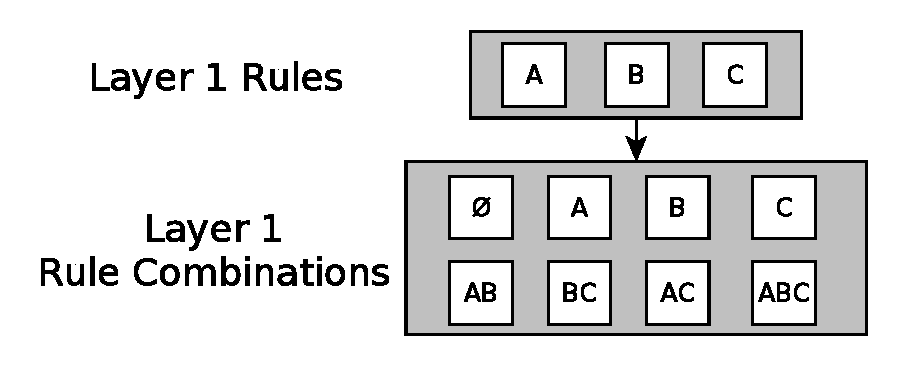
\includegraphics[width=.40\textwidth]{./figures/overview/rule_combos.pdf}
	\caption{Rule combinations created for a transformation layer}
	\label{fig:rule_combos2}
\end{figure}

Note that within these rule combinations, the number of times a rule has
executed is abstracted. Either a rule has executed zero times, and the rule is
not represented in a rule combination, or the rule has executed some finite
number of times and it is represented. This abstraction is key to our approach,
as it allows us to create a finite set of path conditions to abstract over an
infinite set of transformation executions, as seen in
\cref{sec:abstraction_relation}.

We also note that rule \textit{combinations} are created, and not rule
\textit{permutations}. This follows from the semantics of \\DSLTrans as described
in \cref{sec:dsltrans}, as transformation rules in a layer will execute in a
non-deterministic order but produce a deterministic result, by construction of the semantics of DSLTrans. As a final
note, the transformation executions that these rule combinations represent always terminate, also by construction of the semantics of DSLTrans~\cite{DBLP:conf/sle/BarrocaLAFS10}.

We base our concept of path conditions on these rule combinations. However, as
DSLTrans allows for dependencies between rules, we cannot create path conditions
for the transformation by taking the powerset of all rules. Instead, our
approach must move layer-by-layer and resolve the dependencies between rules.
The next two sections will introduce the concepts of traceability and dependency, before we
briefly discuss the syntax and semantics of path conditions themselves.

\subsubsection{Traceability}
\label{subsubsec:traceability}

DSLTrans rules allow for dependencies to be specified on which elements of the
output model were created from specific elements of the input model. To resolve
these dependencies, traceability information for the transformation is created
during the execution of a DSLTrans model transformation~\cite{DBLP:conf/sle/BarrocaLAFS10}.
In our verification approach, we store this same information as symbolic \emph{traceability links}, in
order to record which elements belong to the same DSLTrans rule.


At a particular point in the path condition construction process, symbolic traceability links are built for
each rule as follows: for all match and apply elements of a rule, given a match
element belonging to the match graph of a rule and an apply element belonging to
the apply graph of the same rule, a symbolic traceability link is built between the two
if the apply element is not connected to a backward link (as explained below).
This is intuitive: traceability links are built between a newly generated
element in the output model, and the elements of the input model that originated
it.

\begin{figure}[htb]
        \centering
        \begin{subfigure}[b]{0.24\textwidth}
                \centering
                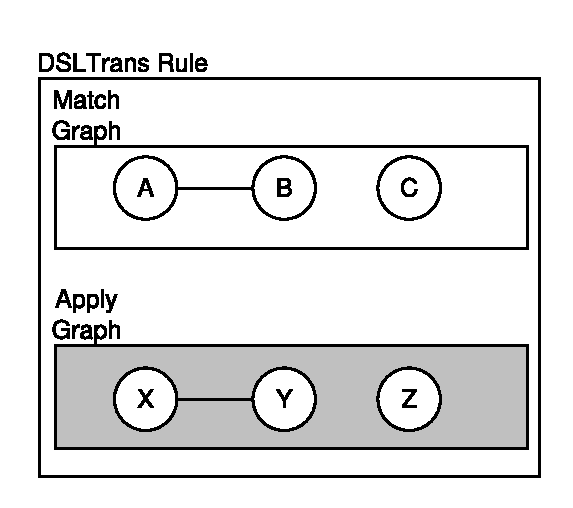
\includegraphics[width=1\textwidth]{./figures/building_path_conditions/traceability_links.pdf}
                \caption{Before symbolic traceability links added}
                \label{fig:traceability_links1}
        \end{subfigure}%
        ~~
        \begin{subfigure}[b]{0.235\textwidth}
                \centering
                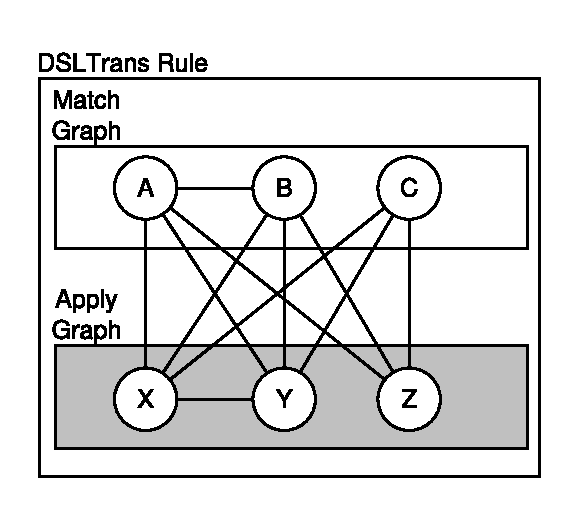
\includegraphics[width=1\textwidth]{./figures/building_path_conditions/traceability_links2.pdf}
                \caption{After symbolic traceability links added}
                \label{fig:traceability_links2}
        \end{subfigure}%
        \caption{Symbolic traceability links created for an abstract DSLTrans rule}
        \label{fig:trace_links}
\end{figure}

An example of the symbolic traceability link creation process is shown in
\cref{fig:trace_links}. Note that symbolic traceability links are a solid line between
match and apply elements in our visual notation.



\subsubsection{Backward Links}
\label{subsubsec:backward_links}

The dependencies in a DSLTrans rule are specified using the \textit{backward link} construct, as further detailed in \cref{subsec:DSLTrans_constructs} and \cref{def:transformation_rule}. \cref{subsubsec:resolve_dependencies} will discuss how these dependencies are then resolved during our symbolic execution approach.

\cref{fig:backward_links} demonstrates how backward links are used \\within a rule. The rule shown contains a backward link, which defines the dependency that an element of type X was created from an element of type A, and an element of type Y was created from an element of type B. If this dependency is satisfied, then another element of type Z should be created. This element should be associated with the Y element.

\begin{figure}[htb]
        \centering
        \begin{subfigure}[b]{0.235\textwidth}
                \centering
                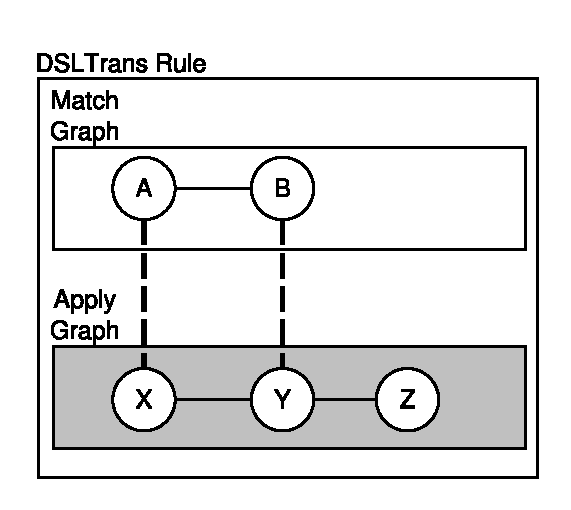
\includegraphics[width=1\textwidth]{./figures/building_path_conditions/backward_link.pdf}
                \caption{Rule with backward links (dashed lines)}
                \label{fig:backward_links}
        \end{subfigure}%
        ~~
        \begin{subfigure}[b]{0.235\textwidth}
                \centering
                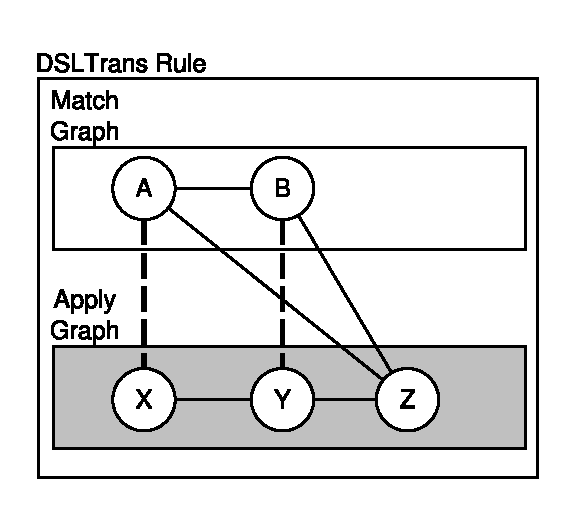
\includegraphics[width=1\textwidth]{./figures/building_path_conditions/backward_link2.pdf}
                \caption{Traceability links added\\~}
                \label{fig:backward_links2}
        \end{subfigure}%
        \caption{Adding traceability links to an abstract DSLTrans rule with backward links}
        \label{fig:back_links}
\end{figure}

\cref{fig:backward_links2} shows the rule after symbolic traceability links have been added. Two symbolic traceability links are created from the Z element to the A and B elements in the match graph to store traceability information. Note that no symbolic traceability links are built between two elements connected by backward links, as these links have already been built in a previous layer.



% \begin{definition}{Rule Traceability}
% 
% Let $rl = \big\langle V,E,st,\tau \big\rangle$ be a transformation
% rule. $trace_{\langle
% V_{\Delta},E_{\Delta},st_{\Delta},\tau_{\Delta}\rangle}(\langle
% V,E,st,\tau\rangle) = \langle V,E',st',\tau'\rangle$ where we have that
% $E\subseteq E'$, $st\subseteq st'$, $\tau \subseteq \tau'$ and if
% $v_1\xrightarrow{e} v_2\in E'\setminus E$ then $v_1\in Output(V_{\Delta})$,
% $v_2\in Input(V)$ and $\tau'(e)=trace$.
% \end{definition}


\subsubsection{Syntax and Semantics}
\label{subsubsec:path_condition_creation}

A path condition represents the symbolic execution of a set of DSLTrans rules, similar to a rule combination as explained above. Again, we use an abstraction over the number of times a rule has symbolically executed. Each path condition will represent that a rule has not executed, or has executed one or more times.

The path condition generation algorithm will symbolically combine transformation rules into a path condition. Each path condition will then abstract a set of concrete transformation executions, as defined by our abstraction relation in \cref{sec:abstraction_relation}.

As seen in the rest of this section, the structure of path conditions is similar to that of DSLTrans rules. The match graph of a path condition represents a pattern that must be present in the input model of the transformation, while the apply graph is a pattern which will be instantiated in the output model of the transformation. Symbolic traceability links are also kept between elements in the match and apply graphs to retain traceability information.

The formal definition of a path condition is presented in \cref{def:path_condition}.

\begin{definition}{Path Condition\\}
\label{def:path_condition}
\CatchFileBetweenTags{\pcdef}{text/definitions}{pcdef}{\pcdef}
\end{definition}

\CatchFileBetweenTags{\pc}{text/definitions}{pc}{\pc}

\subsection{Path Condition Generation Algorithm}
\label{sec:gen_all_pcs}

 This section will describe how path conditions are constructed for a DSLTrans transformation using our approach.

\cref{fig:next_layer} outlines the path condition generation algorithm. The algorithm will examine each transformation layer in turn. Path conditions from the previous layer will be combined with rules from the current layer to create a new set of path conditions. This new set of path conditions will then be combined with the rules from the next layer to produce yet another set of path conditions, and so on. At the end of the algorithm, a complete set of path conditions for the entire transformation will have been produced. 

\begin{figure*}[htb]
        \centering
        \begin{subfigure}[b]{0.34\textwidth}
                \centering
                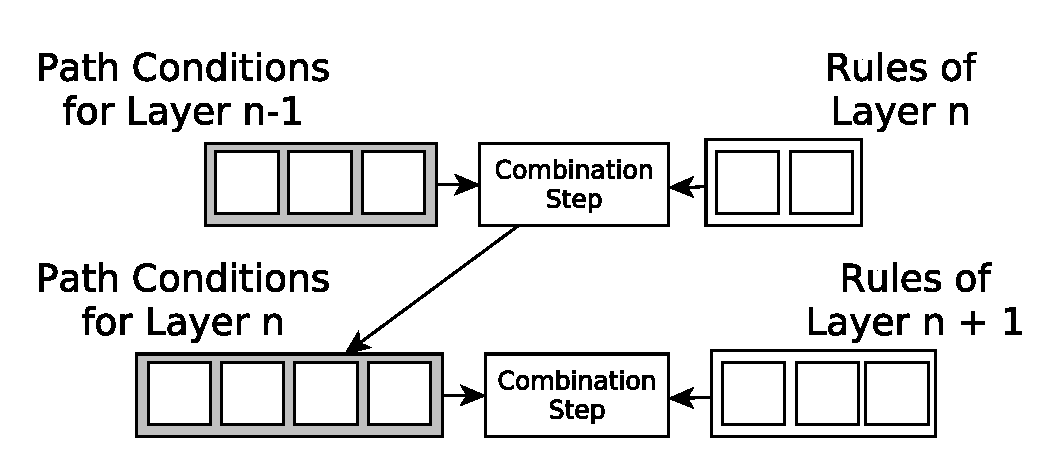
\includegraphics[width=1\textwidth]{./figures/building_path_conditions/next_layer.pdf}
                \caption{Previous path conditions are combined\\ with rules}
                \label{fig:next_layer}
        \end{subfigure}%
        ~~
        \begin{subfigure}[b]{0.34\textwidth}
                \centering
                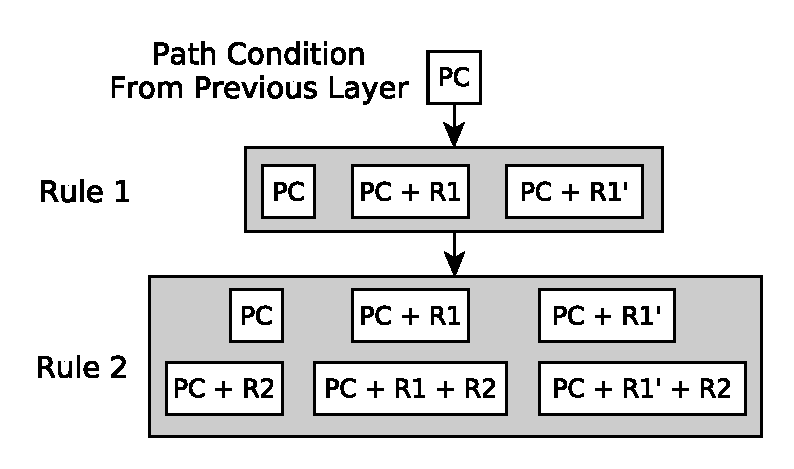
\includegraphics[width=1\textwidth]{./figures/overview/layers_pc.pdf}
                \caption{Combining a path condition with two rules\\~}
                \label{fig:layers_pc2}
        \end{subfigure}%
        
       
         \caption{Two components in the path condition creation process}
         \label{fig:combining_path_conditions}
\end{figure*}

We now define what is occurring in the `combination step' in \cref{fig:next_layer}. This step begins by selecting each path condition in the working set, one at a time. Note that at the beginning of the path condition creation process, this working set consists of an empty path condition.

A new set of path conditions will then be created by sequentially combining each rule in the layer with the path condition selected. Recall that a path condition represents a set of rules that have symbolically executed, thereby abstracting a set of transformation executions through our abstraction relation. Combining a path condition with a rule will produce one or more path conditions depending on how the rule combines with the rules already represented by the path condition. The pre- and post- conditions defined by the path condition will be modified according to the elements found in that rule. 

Each of the new path conditions created from combining a rule with a path condition will then be combined with the next rule in the layer. A small example is shown in \cref{fig:layers_pc2}, where a path condition is combined with two rules. Note that a rule can combine with a path condition in multiple ways (differentiated by prime marks in the figure). \Cref{fig:all_pcs2} shows how path conditions from the previous layer are sequentially combined with all the rules from the current layer. All the path conditions for the layer are then collected to produce the final working set of path conditions for the layer.

        \begin{figure}[bht]
                 \centering
                  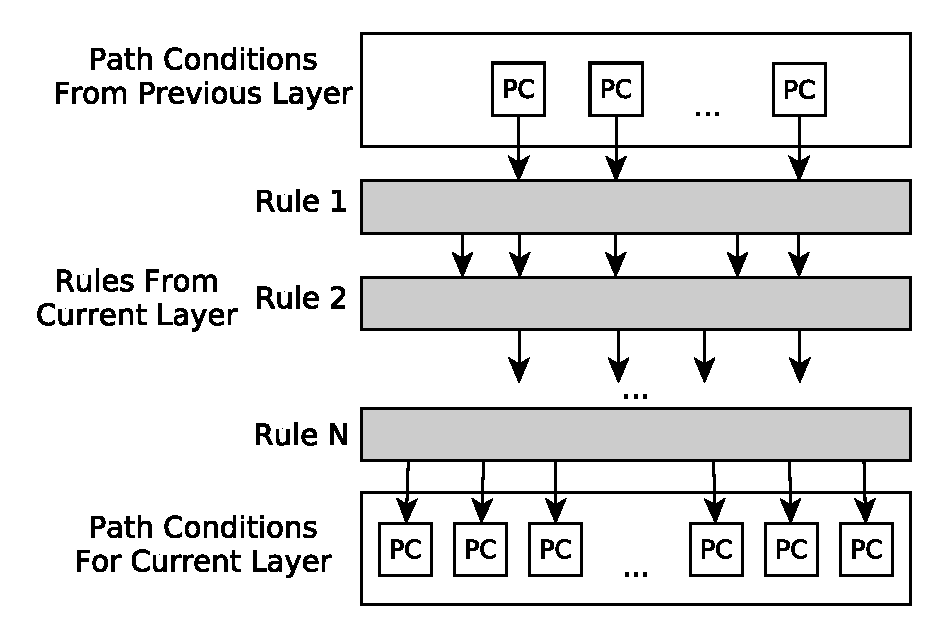
\includegraphics[width=.38\textwidth]{./figures/overview/all_pcs.pdf}
                 \caption{Creating all path conditions for a layer}
                 \label{fig:all_pcs2}
         \end{figure}
         
\subsection{Combining a Path Condition with a Rule}
We will now examine the combination step between one path condition and one rule, which produces a set of new path conditions. A formal and generic definition of this step will be presented first, before we explain the specialized combination possibilities with figures and informal text.

\begin{definition}{Combination of a Path Condition with a Rule}
\label{def:combine_pc_with_rule}

\CatchFileBetweenTags{\pccfrc}{text/definitions}{pccfrc}{\pccfrc}
\end{definition}

\CatchFileBetweenTags{\pccfrctext}{text/definitions}{pccfrctext}{\pccfrctext}

We will now discuss the combination step possibilities. Let PC be the path condition selected from layer n-1, and R the rule selected from layer n. When PC and R are combined, there are four possibilities based on the dependencies between PC and R:

\begin{enumerate}
\item R has \textbf{no} dependencies
\item R has dependencies and \textbf{cannot} execute
\item R has dependencies and \textbf{may} execute
\item R has dependencies and \textbf{will} execute
\end{enumerate}

These dependencies are defined by the backward links within R. As mentioned in \cref{subsubsec:traceability}, backward links enforce that the elements in the apply graph were created by the connected elements in the match graph. In the context of combining a rule and a path condition, these backward links define dependencies between the rule and the elements created by the rules represented by the path condition. 

The below figures will demonstrate the four cases above. As a reminder of visual notation, the backward links are dashed lines between the match and apply graphs of the rule and path condition, while symbolic traceability links are solid lines between the two graphs.

\subsubsection{No Dependencies}
\label{enum:no_back}

The rule R has a match graph which represents its pre-conditions. For a particular transformation execution, it is possible that this match graph would not match a specific input model, and thus R would not execute in these transformation executions. To represent all such transformation executions where the rule R would not execute, PC is copied unchanged to the new set of path conditions.

To represent the transformation executions where the match graph of R would match, and therefore R would execute, a new path condition is produced which consists of the union between R and PC. This situation is
seen in \cref{fig:no_dependencies} and formally defined in \cref{def:rule_comb_no_dependencies}.

\begin{figure}[bt] \centering 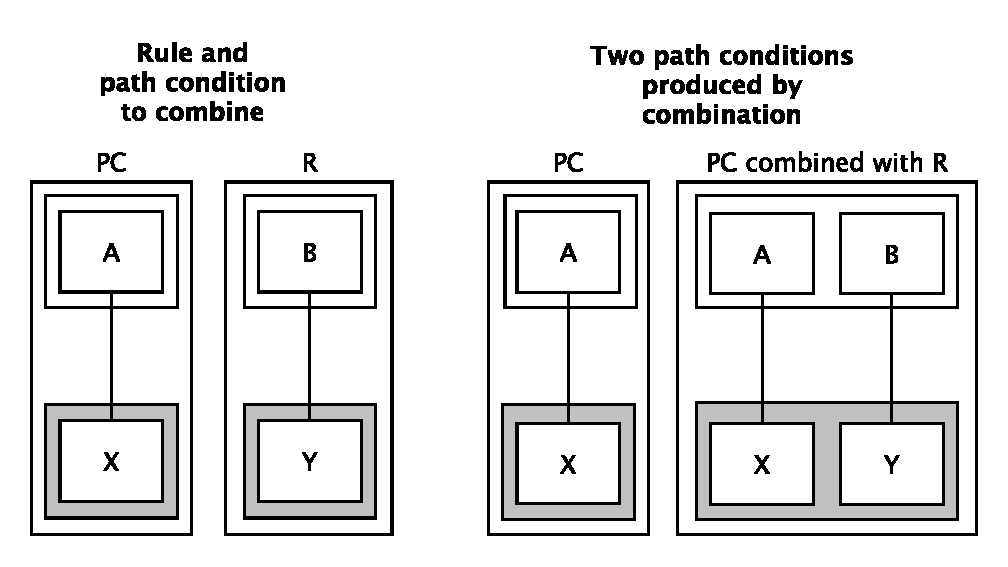
\includegraphics[width=0.44\textwidth]{./figures/building_path_conditions/no_dependencies.pdf}
	\caption{R has no dependencies}
	\label{fig:no_dependencies}
\end{figure}

% \begin{definition}{No Dependencies Between a Rule and a Path Condition}
% 
% \levi{FIX}
% Let $A=\langle V,E,st,\tau\rangle, B=\langle V',E',st',\tau'\rangle\in \textsc{Pathcond}^{sr}_{tg}$ be two path conditions. We say that $R$ does not depend on $PC$ if and only if $\nexists e\in E'\,.\,\tau'(e)=backward$.
% \end{definition}

\begin{definition}{Path Condition and Rule Combination -- No Dependencies\\}
\label{def:rule_comb_no_dependencies}
\CatchFileBetweenTags{\nodeps}{text/definitions}{nodeps}{\nodeps}

\end{definition}

\CatchFileBetweenTags{\nodepstext}{text/definitions}{nodepstext}{\nodepstext}

\subsubsection{Resolving Dependencies}
\label{subsubsec:resolve_dependencies}
If R contains backward links and thus R defines dependencies on PC, then we need to analyse whether PC can satisfy those dependencies. This is done by matching the backward links in R over the symbolic traceability links in PC. Note that symbolic traceability links in R are not required to be found in PC, and that only backward links define dependencies.

\paragraph{Unsatisfied Dependencies}


If the backward links in R cannot be matched to symbolic traceability links in PC, then in the transformation executions abstracted by PC, R cannot execute. Again, PC will be copied unchanged to the new set of path conditions, but no new path condition will be created. This case is shown in \cref{fig:non_satisfied_dependencies}, where the backward links between the two B elements in R cannot match over the symbolic traceability link in PC. \cref{def:rule_comb_unsatisfied} describes this case formally.

\begin{figure}[h!] \centering 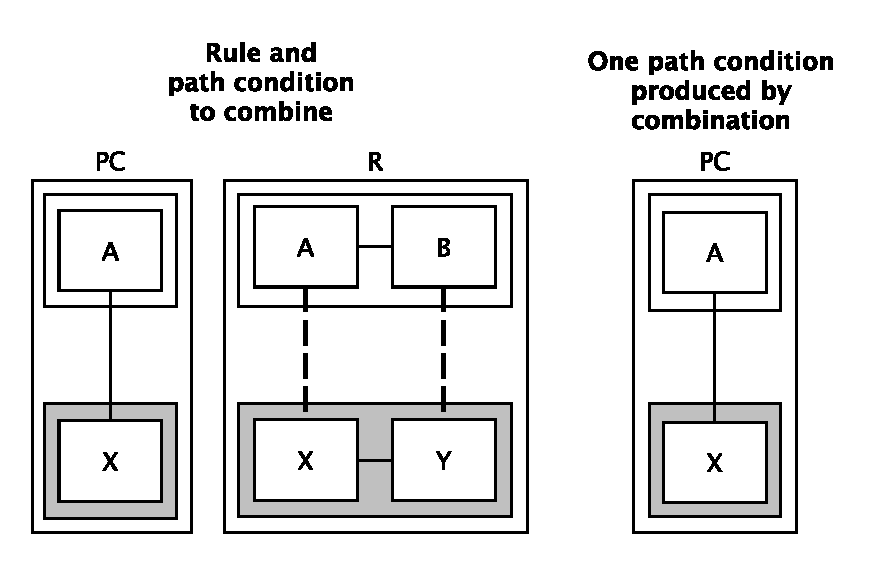
\includegraphics[width=0.44\textwidth]{./figures/building_path_conditions/non_satisfied_dependencies.pdf}
	\caption{R's dependencies are not satisfied by PC}
	\label{fig:non_satisfied_dependencies}
\end{figure}

\begin{definition}{Path Condition and Rule Combination -- Unsatisfied Dependencies\\} 
\label{def:rule_comb_unsatisfied}
\CatchFileBetweenTags{\unsatdeps}{text/definitions}{unsatdeps}{\unsatdeps}
\end{definition}

According to the pre-conditions of the equation presented in \cref{def:rule_comb_unsatisfied}, a path condition does not satisfy the dependencies present in a rule if there is no surjective typed graph homomorphism between the backward links of the rule and the symbolic traceability links of the path condition. Besides expressing the fact that all backward links must exist as symbolic traceability links the path condition, the surjective homomorphism allows modeling the case where dependencies expressed by two (or more) backward links between similarly typed elements can be satisfied one single symbolic traceability link in the path condition. This is the case, for example, of rule \emph{FemaleToFemale} in the \emph{Police Station} in \cref{fig:dsltransformation}. The two similarly typed backward links in this rule are satisfied by a path condition containing only the rule \emph{females} generated from the first layer of the transformation, holding one single symbolic traceability link.


\paragraph{Partially- and Totally- Satisfied Dependencies}

Consider the possibility that the backward links of R can be found in PC, and R's dependencies are met. The question then becomes whether the rule R \textbf{may} or \textbf{will} execute in the abstracted transformation executions.

To resolve this question, the match graph of R, along with R's backward links, is matched to PC's match graph and traceability links. If all of these elements are found, then we denote this as the `totally-satisfied case', where R \textbf{will} necessarily execute in the abstracted transformation executions. Otherwise, we denote the `partially-satisfied' case, where R \textbf{may} execute. Note that we break up these cases for ease of explanation only. Formally, both cases are encompassed by \cref{def:rul_comb_partial_total}.

In the totally-satisfied case, R will be ``glued'' overtop PC, as seen in \cref{fig:total_satisfied_dependencies}. This gluing operation is anchored where the backwards links in R match over the traceability links in PC. The purpose of this operation is to include any elements in R's apply graph that may not exist in PC. Thus, all elements and associations which exist in both PC and R are ignored. Note that if multiple total matches exist in PC, that R will be glued at multiple points as seen in \cref{fig:multiple_total_satisfied_dependencies}. This ``gluing'' operation is also defined formally in \cref{def:rul_comb_partial_total}, as the addition of a delta graph.

\begin{figure*}[htb]
        \centering
        \begin{subfigure}[b]{0.7\textwidth}
                \centering
                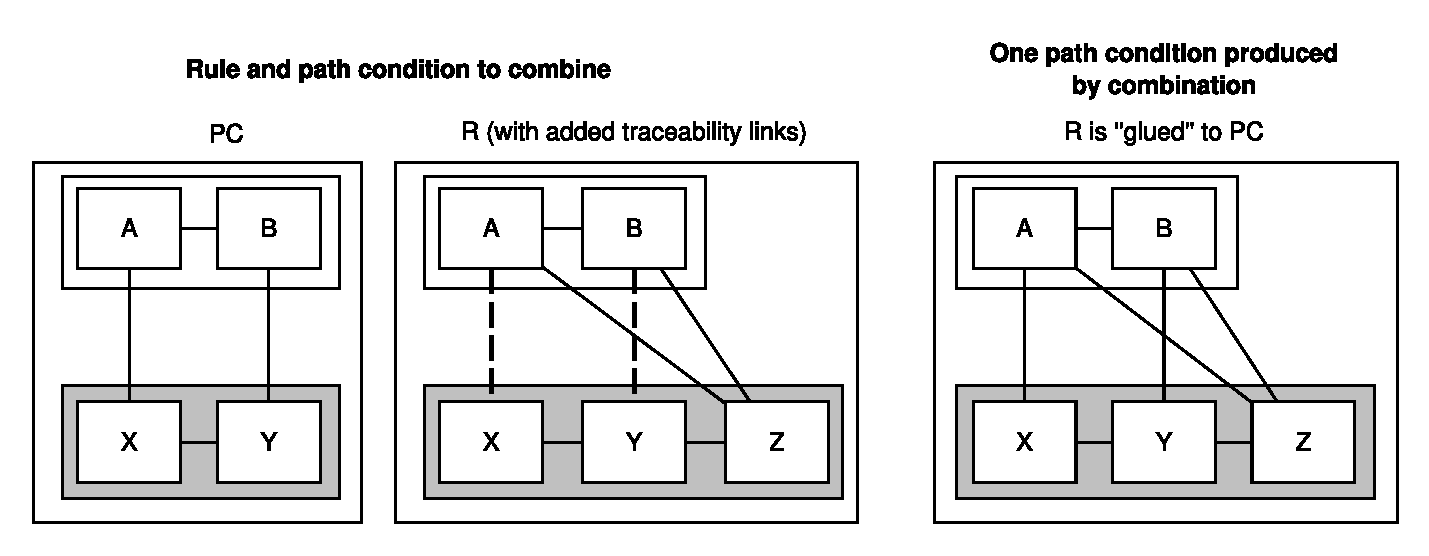
\includegraphics[width=1\textwidth]{./figures/building_path_conditions/total_satisfied_dependencies.pdf}
                \caption{Totally satisfied at one location}
                \label{fig:total_satisfied_dependencies}
        \end{subfigure}%
        \\
        \begin{subfigure}[b]{0.8\textwidth}
                \centering
                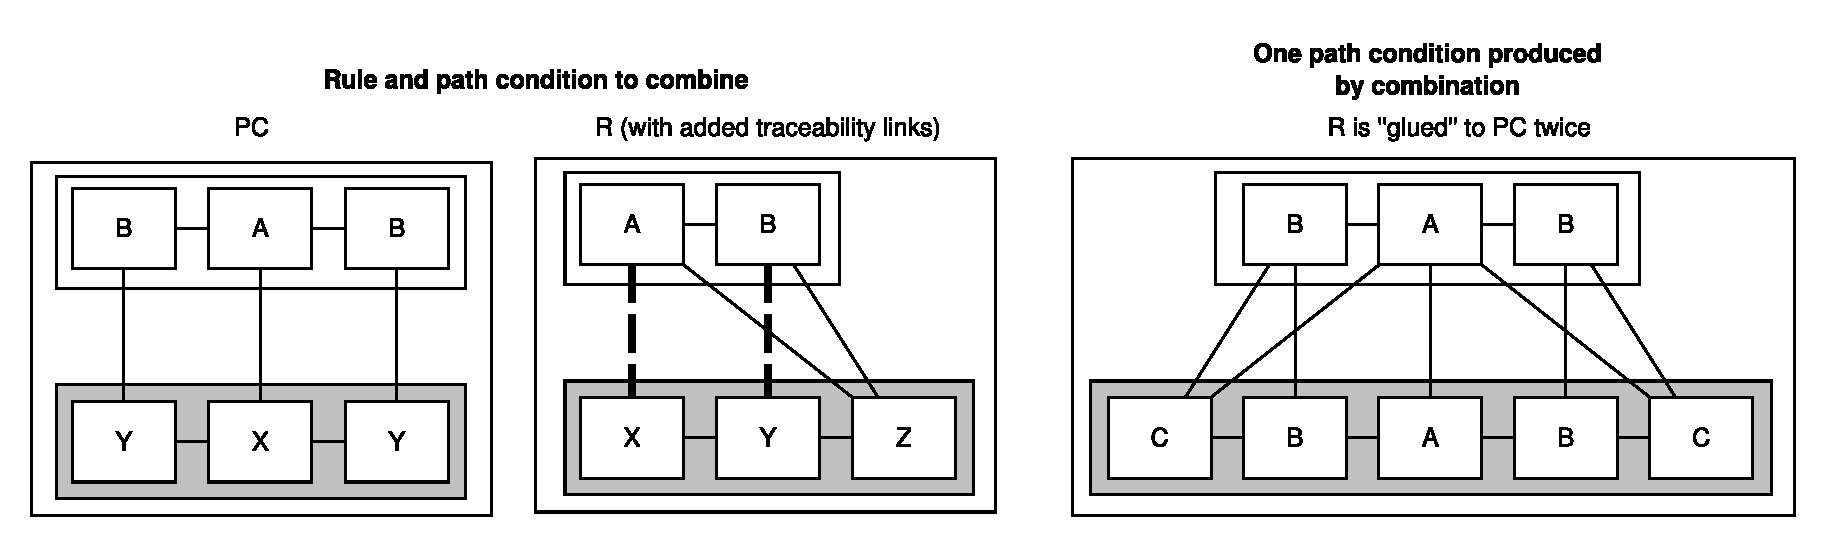
\includegraphics[width=1\textwidth]{./figures/building_path_conditions/multiple_total_satisfied_dependencies.pdf}
                \caption{Totally satisfied at multiple locations}
                \label{fig:multiple_total_satisfied_dependencies}
        \end{subfigure}%
        \caption{R's dependencies are totally satisfied by PC}
        \label{fig:totes_sat_deps}
\end{figure*}

In the partially-satisfied case, rule R may or may not execute. Note that in \cref{fig:partial_satisfied_dependencies}, PC does not have the association between the A and B elements in the match graph. This means that it is possible that the input model for the transformation does not have this association present. In these transformation executions R would not execute.
\cref{fig:partial_satisfied_dependencies} shows the two path conditions produced in this case. The first produced is a copy of PC, where R does not symbolically execute. The second is where R symbolically executes at the matched location. Therefore, R is glued onto PC, with the gluing step the same as in the totally-satisfied case above.

\begin{figure*}[tb] \centering 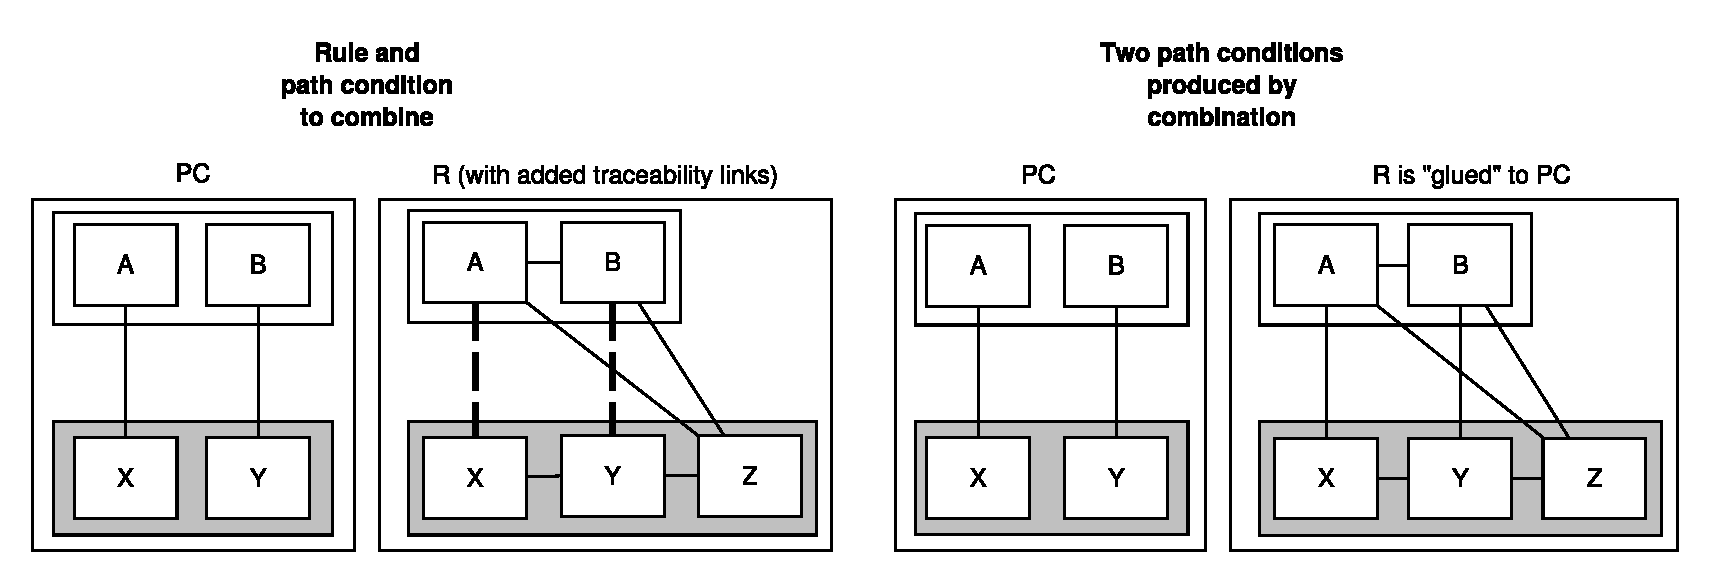
\includegraphics[width=0.8\textwidth]{./figures/building_path_conditions/partial_satisfied_dependencies.pdf}
	\caption{R's dependencies are partially satisfied by PC}
	\label{fig:partial_satisfied_dependencies}
\end{figure*}

Note that this gluing procedure must consider all matching possibilities, for each location the rule might match over the input model. For example, in \cref{fig:multiple_partial_satisfied_dependencies}, rule R has a backward link that can be partially matched on two locations in PC: the left-hand and right-hand pairs of traceability links. Therefore, there are four possibilities for how R would match over PC: not at all, on the left-hand side of PC, on the right-hand side, or on both sides. These four possibilities define the four new path conditions created.

The first is a copy of PC, as R is assumed to not execute and will produce no new elements. The second is where R will be glued on top of the backward links on the left-hand side, to add the elements that do not exist in PC already. The third is where the gluing will occur on the right-hand side. The fourth path condition produced is the case where R will be glued at both locations. 


\begin{figure*}[tb] \centering 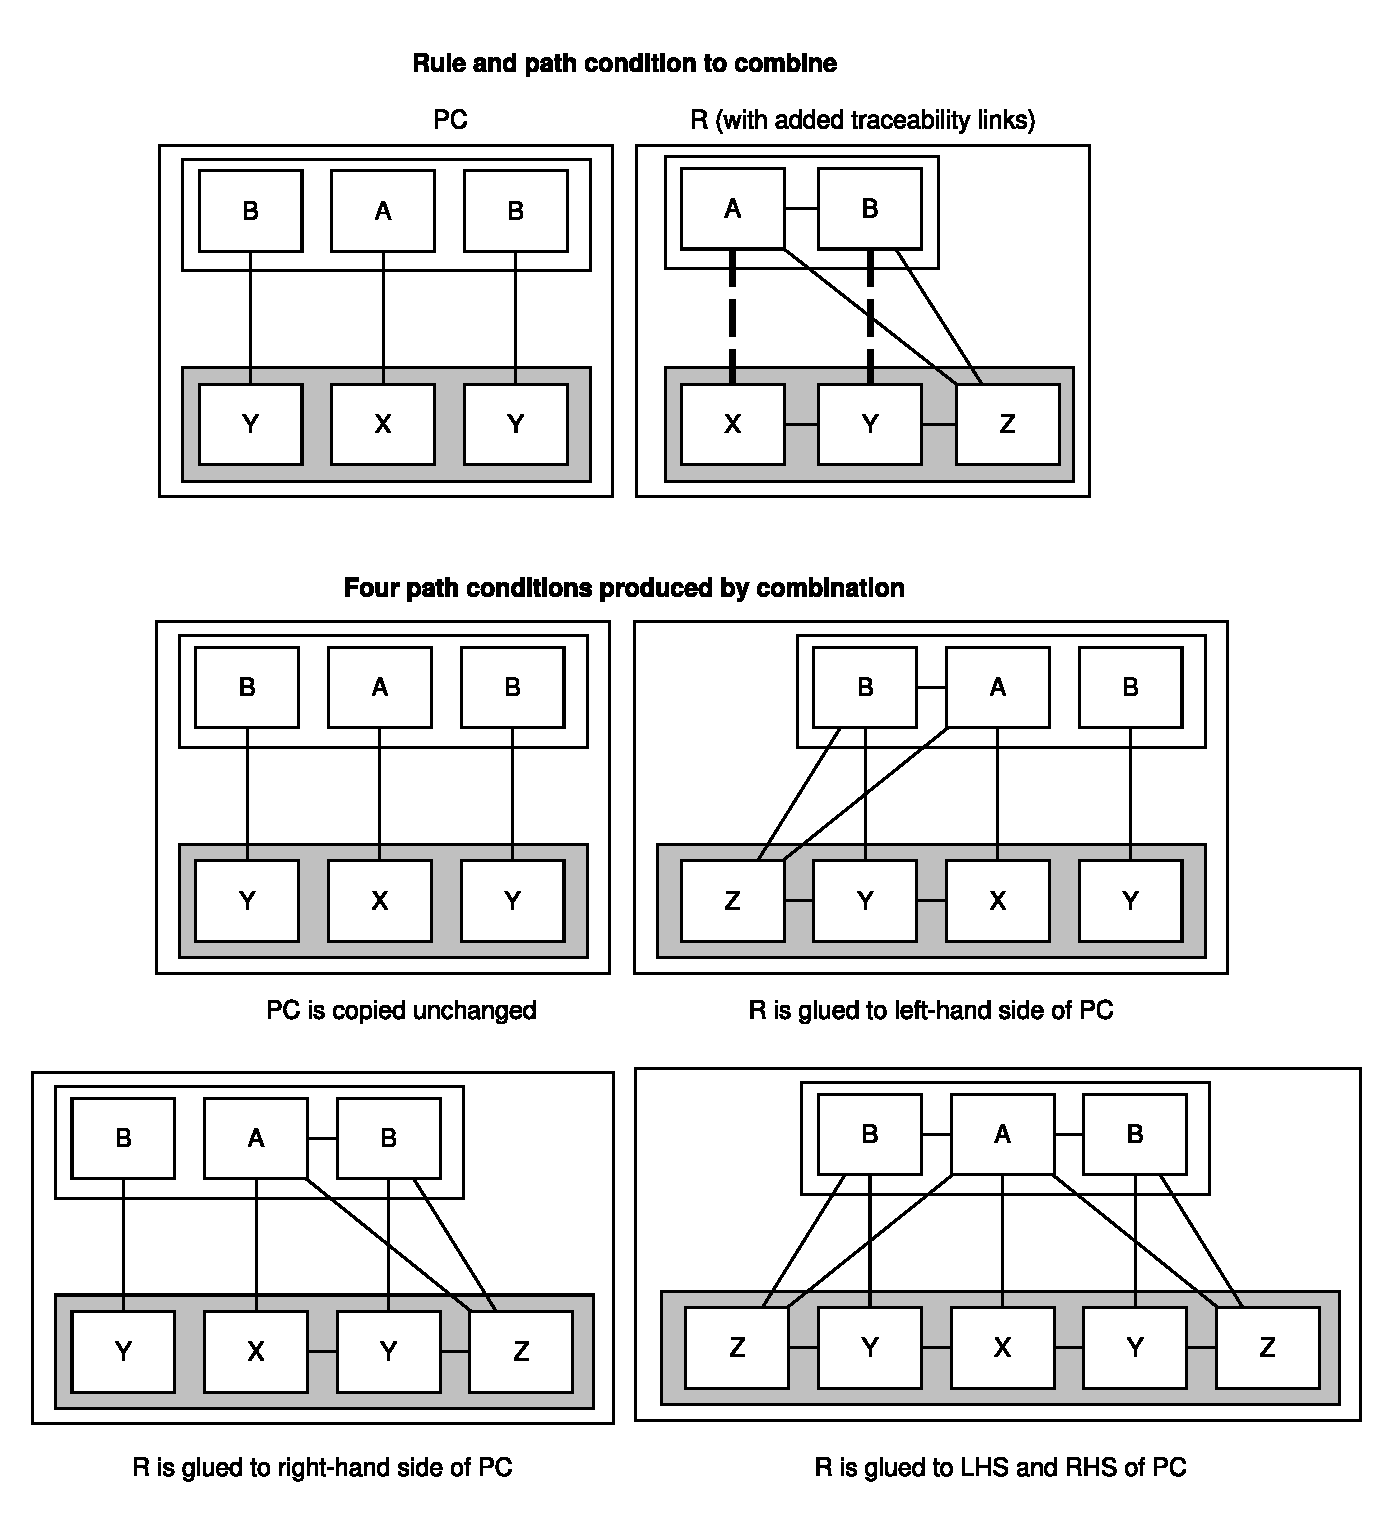
\includegraphics[width=0.8\textwidth]{./figures/building_path_conditions/multiple_partial_satisfied_dependencies.pdf}
	\caption{R's dependencies are partially satisfied by PC, and are glued at all possible matches}
	\label{fig:multiple_partial_satisfied_dependencies}
\end{figure*}


Note that rules may also contain transitive links in their match graphs. In this case, the partial or total matching of R onto PC must consider all transitive matches in order to produce all valid path conditions.

As we have done for the previous cases, let us now formally define the combination step when a rule has partially and/or totally defined dependencies. As these cases are more complex than the previous two, we will need to construct the mathematical model of this case incrementally. We will start by an auxiliary relation that partially or totally combines a set of path conditions with a rule.

\begin{definition}{Single Partial and Total Combination of a Set of Path Conditions with a Rule\\}
\label{def:comb_path_cond_rule_single}
\CatchFileBetweenTags{\satdeps}{text/definitions}{satdeps}{\satdeps}

\begin{align}
\label{eq:pcomb}
\CatchFileBetweenTags{\satdepseqone}{text/definitions}{satdepseqone}{\satdepseqone}
\end{align}


\begin{align}
\label{eq:tcomb}
\CatchFileBetweenTags{\satdepseqtwo}{text/definitions}{satdepseqtwo}{\satdepseqtwo}
\end{align}

\end{definition}


Let us start by introducing relation $\stackrel{p\_comb}{\rightarrow}$, presented in \cref{eq:pcomb} of \cref{def:comb_path_cond_rule_single}. The relation takes as arguments a set of path conditions being accumulated for the current layer, the rule to be combined, and an $rl_{glue}$ argument indicating the place in each of the input path conditions the rule should be anchored to during the combination step. The relation's output is a new set of path conditions. This new set includes all the original path conditions, as well as each path condition in the accumulator set ``glued'' to a copy of rule being examined. Note that the relation $\stackrel{t\_comb}{\rightarrow}$ in \cref{eq:tcomb} of \cref{def:comb_path_cond_rule_single} is similarly defined, except for the fact path conditions in the accumulator set are not preserved in the relation's output set.\\

\setcounter{equation}{0} 

Let us now define how a rule is combined with a path condition, whenever its backward links can be found several times in that path condition. This situation is described in the examples in \cref{fig:multiple_total_satisfied_dependencies} and \cref{fig:multiple_partial_satisfied_dependencies}. We formalize it in \cref{def:comb_path_cond_rule_mul}, by means of relations $\stackrel{p\_step}{\rightarrow}$ and $\stackrel{t\_step}{\rightarrow}$. These two relations operationally describe the sequence of steps necessary to ``glue'' a rule at multiples places of a path condition. The set of places targeted in the path condition for receiving a copy of the rule is given by the sets $partialSet$ and $totalSet$ (found respectively in Equation~(2) and Equation~(4) of \cref{def:comb_path_cond_rule_mul}). As expected, these sets contain the set of traceability links in the path condition where copies of the rule need to be anchored to.

\begin{definition}{Multiple Partial and Total Combination of a Set of Path Conditions with a Rule\\}
\label{def:comb_path_cond_rule_mul}

\CatchFileBetweenTags{\satdepstwo}{text/definitions}{satdepstwo}{\satdepstwo}
\end{definition}

Having \cref{def:comb_path_cond_rule_single} and \cref{def:comb_path_cond_rule_mul} in mind, we can now proceed to define the complete combination relation of a rule with a path condition in the case of partially and totally satisfied dependencies. 

\begin{definition}{Path Condition and Rule Combination -- Partially and Totally Satisfied Dependencies\\}
\label{def:rul_comb_partial_total}

\CatchFileBetweenTags{\satdepsthree}{text/definitions}{satdepsthree}{\satdepsthree}
\end{definition}

The top equation in \cref{def:rul_comb_partial_total} defines the $\stackrel{combine}{\rightarrow}$ relation for when rule $rl$ has dependencies that are satisfied by path condition $pc$. The pre-conditions in the equation state that the backward links in the rule are found in the path condition, as expected. Additionally, two sequential steps perform the gluing of the rule $rl$ on all path conditions in accumulator $AC$, wherever the rule is partially and/or totally found in each of those path conditions. Relations $\stackrel{p\_comb}{\rightarrow}$ and $\stackrel{t\_comb}{\rightarrow}$ presented in \cref{def:comb_path_cond_rule_mul} are used to model these two operational ``gluing'' steps. Functions $partialsat$ and $totalsat$, described in the latter part of \cref{def:rul_comb_partial_total}, are used to gather the places of path condition $pc$ where copies of the rule need to be anchored to.


\subsubsection{Considering Further Rules}
\label{sec:further_rules}
Thus far we have described how to create a set of path conditions that represent how one rule from a layer will add new elements to one path condition from the previous layer. These path conditions are then themselves combined with the next rule in the layer in the same manner. Note that in \cref{def:rul_comb_partial_total} the choice of next rule does not matter, due to the rule non-interference guaranteed by the semantics of DSLTrans. In order to represent this non-interference in the construction of path conditions, we specify that the matching of rule dependencies is against the path condition from the previous layer (variable $pc$ in the main equation of \cref{def:rul_comb_partial_total}), not the specific path condition the rule is to be combined with in the accumulator argument of the $\stackrel{combine}{\rightarrow}$ relation. This ensures that the result of combining one rule with a path condition will have no impact on how following rules will combine.

% Note that the choice of next rule does not matter, due to the rule non-interference guaranteed by the semantics of DSLTrans. In order to represent this non-interference in the construction of path conditions, we specify that the matching of rule dependencies is against the path condition from the previous layer, not the specific path condition the rule is to be combined with. This ensures that the result of combining one rule with a path condition will have no impact on how following rules will combine.

The combination of one path condition with all the rules in the layer will produce a new set of path conditions. This process is depicted in \cref{fig:all_pcs2} and formalized in \cref{def:path_cond_layer_comb} by the layer combination relation $\stackrel{combpclayer}{\rightarrow}$.

\begin{definition} {Combining a Path Condition with a Layer\\}
\label{def:path_cond_layer_comb}
\CatchFileBetweenTags{\combpclayer}{text/definitions}{combpclayer}{\combpclayer}
\end{definition}

\CatchFileBetweenTags{\combpclayertext}{text/definitions}{combpclayertext}{\combpclayertext}

\begin{definition} {Combining a Set of Path Conditions with a Layer\\}
\label{def:path_cond_set_layer_comb}
\CatchFileBetweenTags{\combpcsetlayer}{text/definitions}{combpcsetlayer}{\combpcsetlayer}
\end{definition}

\CatchFileBetweenTags{\combpcsetlayertext}{text/definitions}{combpcsetlayertext}{\combpcsetlayertext} 

\begin{definition} {Path Condition Generation\\}
\label{def:path_cond_gen}
\CatchFileBetweenTags{\pathcondgen}{text/definitions}{pathcondgen}{\pathcondgen}
\end{definition}

\CatchFileBetweenTags{\pathcondgentext}{text/definitions}{pathcondgentext}{\pathcondgentext} 





